\documentclass[11pt]{article}

% Language setting
\usepackage[turkish]{babel}
\usepackage{pythonhighlight}

\usepackage[a4paper,top=2cm,bottom=2cm,left=2cm,right=2cm,marginparwidth=2cm]{geometry}

% Useful packages
\usepackage{amsmath}
\usepackage{graphicx}
\usepackage[colorlinks=true, allcolors=blue]{hyperref}
\usepackage{verbatim}
\usepackage{fancyhdr} % for header and footer
\usepackage{titlesec}
\usepackage{parskip}

\setlength{\parindent}{0pt}

\titleformat{\subsection}[runin]{\bfseries}{\thesubsection}{1em}{}

\pagestyle{fancy} % activate the custom header/footer

% define the header/footer contents
\lhead{\small{23BLM-4014 Yapay Sinir Ağları Ara Sınav Soru ve Cevap Kağıdı}}
\rhead{\small{Dr. Ulya Bayram}}
\lfoot{}
\rfoot{}

% remove header/footer on first page
\fancypagestyle{firstpage}{
  \lhead{}
  \rhead{}
  \lfoot{}
  \rfoot{\thepage}
}
 

\title{Çanakkale Onsekiz Mart Üniversitesi, Mühendislik Fakültesi, Bilgisayar Mühendisliği Akademik Dönem 2022-2023\\
Ders: BLM-4014 Yapay Sinir Ağları/Bahar Dönemi\\ 
ARA SINAV SORU VE CEVAP KAĞIDI\\
Dersi Veren Öğretim Elemanı: Dr. Öğretim Üyesi Ulya Bayram}
\author{%
\begin{minipage}{\textwidth}
\raggedright
Öğrenci Adı Soyadı: Nuray Altuğ\\ % Adınızı soyadınızı ve öğrenci numaranızı noktaların yerine yazın
Öğrenci No: 190401056
\end{minipage}%
}

\date{14 Nisan 2023}

\begin{document}
\maketitle

\vspace{-.5in}
\section*{Açıklamalar:}
\begin{itemize}
    \item Vizeyi çözüp, üzerinde aynı sorular, sizin cevaplar ve sonuçlar olan versiyonunu bu formatta PDF olarak, Teams üzerinden açtığım assignment kısmına yüklemeniz gerekiyor. Bu bahsi geçen PDF'i oluşturmak için LaTeX kullandıysanız, tex dosyasının da yer aldığı Github linkini de ödevin en başına (aşağı url olarak) eklerseniz bonus 5 Puan! (Tavsiye: Overleaf)
    \item Çözümlerde ya da çözümlerin kontrolünü yapmada internetten faydalanmak, ChatGPT gibi servisleri kullanmak serbest. Fakat, herkesin çözümü kendi emeğinden oluşmak zorunda. Çözümlerinizi, cevaplarınızı aşağıda belirttiğim tarih ve saate kadar kimseyle paylaşmayınız. 
    \item Kopyayı önlemek için Github repository'lerinizin hiçbirini \textbf{14 Nisan 2023, saat 15:00'a kadar halka açık (public) yapmayınız!} (Assignment son yükleme saati 13:00 ama internet bağlantısı sorunları olabilir diye en fazla ekstra 2 saat daha vaktiniz var. \textbf{Fakat 13:00 - 15:00 arası yüklemelerden -5 puan!}
    \item Ek puan almak için sağlayacağınız tüm Github repository'lerini \textbf{en geç 15 Nisan 2023 15:00'da halka açık (public) yapmış olun linklerden puan alabilmek için!}
    \item \textbf{14 Nisan 2023, saat 15:00'dan sonra gönderilen vizeler değerlendirilmeye alınmayacak, vize notu olarak 0 (sıfır) verilecektir!} Son anda internet bağlantısı gibi sebeplerden sıfır almayı önlemek için assignment kısmından ara ara çözümlerinizi yükleyebilirsiniz yedekleme için. Verilen son tarih/saatte (14 Nisan 2023, saat 15:00) sistemdeki en son yüklü PDF geçerli olacak.
    \item Çözümlerin ve kodların size ait ve özgün olup olmadığını kontrol eden bir algoritma kullanılacaktır. Kopya çektiği belirlenen vizeler otomatikman 0 (sıfır) alacaktır. Bu nedenle çözümlerinizi ve kodlarınızı yukarıda sağladığım gün ve saatlere kadar kimseyle paylaşmayınız.
    \item Bu vizeden alınabilecek en yüksek not 100'dür. Toplam aldığınız puan 100'ü geçerse, aldığınız not 100'e sabitlenecektir.
    \item LaTeX kullanarak PDF oluşturanlar öz geçmişlerine LaTeX bildiklerini de eklemeyi unutmasınlar :)
    \item Bu vizedeki soruların çözümleri ve tex dosyası için istediğiniz kadar sayıda Github repository'si oluşturabilirsiniz. Sadece yukarıda belirttiğim tarihlerde (14 Nisan 2023 saat 15:00 ile 15 Nisan 2023 saat 15:00 arasında) public yapmayı/halka açmayı ve Github profilinizi de öz geçmişinize eklemeyi unutmayın :)
    \item Bilgisayarınıza hiçbir program kurmadan, Overleaf, Google Colab, Kaggle gibi ortamlar üzerinden bu vizeyi tamamlamanız mümkün. İyi çalışmalar!!
\end{itemize}

(Ekstra 5 puan) \url{OdevinTexDosyasınınGithubLinkiniburayakoyun.com}

\newpage
\section{(Toplam 10 Puan) Hopfield Networks:}

\subsection{(2 Puan)} \textbf{ChatGPT’ye size Hopfield Network’ler ile ilgili detaylı bilgi vermesini isteyin. Sorduğunuz soruyu, ChatGPT'nin çıkartığı cevabı aşağı koyun. Bu cevapta anlamadığınız terimleri de ChatGPT’ye sorup, sorduğunuz soruları ve ChatGPT’nin verdiği cevapları da sırayla aşağı koyun.}

  \textbf{+Hopfield network'ler ile ilgili detaylı bilgi verir misin?}
  
  -Elman ve Jordan gibi birçok yapay sinir ağı modeli, sürekli zamanlı dinamiklere dayanırken, Hopfield ağları (Hopfield Networks) çekişmeli veya diskretize dinamiklere dayalıdır. Bu ağlar, modellenen bilginin düğümler arasında depolanması ve hatırlanması için tasarlanmıştır. Bu nedenle, tipik olarak bellek veya tanıma problemleri için kullanılırlar.

Hopfield ağı, bir ağın tam bağlı bir düğüm kümesi olduğu ve her düğümün diğer düğümlerle birbirine bağlandığı bir geri besleme ağıdır. Bu ağ, sadece bir katmana sahiptir ve her düğüm, diğer düğümlere göre ölçülen bir aktivasyon seviyesine sahiptir. Düğümler, belirli bir giriş örneğine veya modelin dahili durumuna göre aktive olurlar.

Hopfield ağı, bir bellek işlevi yerine getirir. Ağ, önceden öğrenilmiş örneklerin bir bellek kaynağı olarak depolanabileceği bir ağ topolojisine sahiptir. Daha sonra, bu bellek kaynağı, örneklerin bir kısmının girildiği bir hatırlama modu sırasında kullanılabilir. Ağ, öğrenilmiş örneklerin, modelin bellek kapasitesi sınırlamaları dahilinde tam olarak hatırlanabileceği ve kısmi girişlere dayalı olarak bir çıkış üretebileceği bir öğrenme işlemine tabi tutulur.

Hopfield ağları aynı zamanda modeldeki asimetrik bağlantıların çıkışa benzer bir aktivasyonla karşılık geldiği bir ağ örneğidir. Ayrıca, her düğümün bir aktivasyon eşiği vardır, bu eşik, düğümün çıktısı için gereken girdi miktarını belirler.

Hopfield ağları, boyutsal azaltma, veri sıkıştırma, görüntü işleme ve belirli bellek görevleri gibi uygulamalarda yaygın olarak kullanılmaktadır. Ancak, ağın bellek kapasitesi ve daha büyük boyutlu girdilerle ilgili performans sınırlamaları vardır.

Sonuç olarak, Hopfield ağları, bellek ve tanıma problemlerini çözmek için özel olarak tasarlanmış geri besleme ağlarıdır ve öğrenme süreci sırasında veri örnekleri bellek kaynağı olarak depolanır ve daha sonra bu bellek kaynağı, kısmi girişlerle hatırlama modu sırasında kullanılabilir.

   \textbf{+Sürekli zamanlı dinamik ve çekişmeli veya diskretize dinamik dediğin şey ne?}

  -Sürekli zamanlı dinamikler ve çekişmeli (discrete-time) veya diskretize (discrete-valued) dinamikler, yapay sinir ağı modellerinin farklı türlerinde kullanılan dinamiklerdir.

Sürekli zamanlı dinamikler, doğrusal veya doğrusal olmayan diferansiyel denklemler şeklinde ifade edilir. Bu tür dinamikler, özellikle kontrol sistemleri veya zamana bağımlı modeller için kullanışlıdır. Sürekli zamanlı dinamiklerde, modeldeki değişkenlerin değerleri sürekli olarak değişir ve belirli bir zaman aralığında ölçülür.

Öte yandan, çekişmeli veya diskretize dinamikler, sistemin her zaman adımında ölçülen bir çıktıyı ifade eden bir dizi non-lineer denklem kullanır. Bu tür dinamikler, özellikle bellek veya tanıma problemleri gibi diskretize verilerle ilgili problemler için kullanılır. Çekişmeli veya diskretize dinamiklerde, modeldeki değişkenlerin değerleri yalnızca belirli zaman adımlarında değişir ve sürekli bir zaman boyunca ölçülmez.

Hopfield ağı, bir çekişmeli dinamik modeldir ve bellek veya tanıma problemlerinde kullanılır. LSTM (Long Short-Term Memory) ve GRU (Gated Recurrent Unit) gibi diğer yapay sinir ağı modelleri, sürekli zamanlı dinamiklere dayalıdır ve özellikle doğal dil işleme ve zaman serileri gibi problemlerde kullanılır.

Genel olarak, modelin kullanım amacına bağlı olarak, sürekli zamanlı dinamikler veya çekişmeli/diskretize dinamiklerden hangisinin kullanılacağına karar verilir.

\textbf{+Kısmi girişlerle hatırlama modu ne zaman ve ne gibi işler için kullanılıyor}

-Kısmi girişlerle hatırlama modu, Hopfield ağları gibi bazı yapay sinir ağı modellerinde kullanılan bir tekniktir. Bu teknikte, modele bir kısmi giriş verilir ve model, bu kısmi girişe uygun bir şekilde tamamlanır. Bu tamamlama işlemi, modele daha önce öğretilmiş olan bir dizi kalıp (pattern) kullanılarak gerçekleştirilir.

Kısmi girişlerle hatırlama modu, bellek veya tanıma problemlerinde kullanılabilir. Örneğin, bir Hopfield ağı modeli, bir yüz resminin sadece bir kısmını (örneğin, gözler, burun ve ağız) alabilir ve bu kısmi girişi kullanarak yüzün tamamını hatırlayabilir. Benzer şekilde, bir Hopfield ağı, bir metin belgesinin sadece bir kısmını (örneğin, başlık ve birkaç cümle) alabilir ve bu kısmi girişi kullanarak belgenin tamamını hatırlayabilir.

Kısmi girişlerle hatırlama modu, özellikle bellek veya tanıma problemlerinde kullanışlıdır çünkü gerçek hayatta sıklıkla karşılaşılan veri eksiklikleriyle başa çıkmak için kullanılabilir. Örneğin, bir yüz tanıma sistemi, yüzün tamamının görünmediği durumlarda (örneğin, yüzün bir kısmı engellenmişse veya yüz sadece bir açıdan görülebiliyorsa) kısmi girişlerle hatırlama modunu kullanarak yüzün tamamını hatırlayabilir.

Bununla birlikte, kısmi girişlerle hatırlama modu, öğrenme sürecinde daha fazla veri işleme ve hesaplama gerektirir, bu da modelin eğitim süresini uzatabilir. Ayrıca, kısmi girişlerle hatırlama modu, bazı durumlarda hatırlama doğruluğunu azaltabilir, çünkü model tamamlama işlemini gerçekleştirirken bir kısmı eksik olan verilerle çalışmak zorunda kalır. Bu nedenle, kullanılacak yapay sinir ağı modeli ve uygulama senaryosu dikkatle değerlendirilmelidir.

\textbf{+Çok kullanılan bir yöntem midir?}

-Kısmi girişlerle hatırlama modu, Hopfield ağları gibi yapay sinir ağı modellerinde sıklıkla kullanılan bir tekniktir. Bu nedenle, bellek veya tanıma problemleri gibi birçok farklı uygulama alanında yaygın olarak kullanılmaktadır.

Ancak, kısmi girişlerle hatırlama modu her zaman en iyi seçenek olmayabilir. Kısmi girişlerle hatırlama modu, öğrenme sürecinde daha fazla hesaplama ve veri işleme gerektirir, bu da eğitim süresini uzatabilir. Ayrıca, kısmi girişlerin hatırlama doğruluğunu azaltabileceği de göz önünde bulundurulmalıdır.

Bu nedenle, hangi hatırlama yönteminin kullanılacağı, verilerin doğası, boyutu ve özellikleri gibi faktörlere bağlı olacaktır. Hangi yöntemin en iyi sonuçları vereceğine karar vermek için, uygulama senaryosunun dikkatli bir şekilde değerlendirilmesi ve farklı yöntemlerin karşılaştırılması gerekmektedir.


\textbf{+Hopfield networks çok kullanılıyor mu ve gerçek hayatta nerelerde kullanılıyor?}

Hopfield ağları, yapay sinir ağı alanında önemli bir model olarak kabul edilir ve özellikle bellek ve hatırlama gibi uygulamalarda kullanılır. Hopfield ağları, bir bellek fonksiyonu olarak kullanılabildiği için, bellek ve veri hatırlama problemlerinin çözümünde önemli bir rol oynarlar. Ayrıca, optimizasyon problemlerinin çözümünde de kullanılabilirler.

Gerçek hayatta, Hopfield ağları birçok uygulama alanında kullanılabilir. Örneğin, bellek ve hatırlama problemlerinde kullanıldığından, biyometrik tanıma, yüz tanıma ve parmak izi tanıma gibi alanlarda kullanılabilirler. Hopfield ağları ayrıca, özellikle NP-zor problemlerinde kullanılan bir optimizasyon algoritması olarak kullanılabilirler.

Hopfield ağları ayrıca, devre tasarımı, robotik ve yapay zeka gibi birçok uygulama alanında kullanılır. Örneğin, devre tasarımı alanında, Hopfield ağları, otomatik olarak tasarlanmış analog devrelerin optimizasyonu ve tasarımı için kullanılabilir. Robotik alanında, Hopfield ağları, robotların pozisyon ve hareket kontrolü için kullanılabilir.

Sonuç olarak, Hopfield ağları birçok farklı uygulama alanında kullanılan önemli bir yapay sinir ağı modelidir ve bellek, optimizasyon, biyometrik tanıma, devre tasarımı, robotik ve yapay zeka gibi birçok alanda kullanılabilirler.

\textbf{+Sen geliştirilirken kullandılar mı peki? }

Ben bir yapay zeka modeliyim ve OpenAI tarafından geliştirildim. Dolayısıyla benim geliştirilmesinde birçok farklı teknoloji, algoritma ve araç kullanıldı. Ancak benim geliştirilmesi sırasında Hopfield ağları doğrudan kullanılmadı. Bununla birlikte, Hopfield ağları gibi diğer yapay sinir ağı modelleri benzer teknikler ve algoritmalar kullanır ve yapay zeka alanındaki gelişmeler genellikle birbirlerini tamamlar.

\textbf{+Şifreleme, el yazı tanımlama, örüntü tamamlama vb gibi şeylerde kullanılıyor mu?}

-Evet, Hopfield ağları şifreleme, el yazısı tanıma, örüntü tamamlama ve diğer birçok uygulama alanında kullanılabilir.

Örneğin, Hopfield ağları şifreleme problemlerinin çözümünde kullanılabilirler. Ağın sinir hücreleri, giriş verilerini alır ve verileri belirli bir düzende sıralar. Bu düzenleme işlemi, verilerin şifrelenmesini sağlar. Aynı şekilde, Hopfield ağları, el yazısı tanıma gibi uygulamalarda da kullanılabilir. Ağ, önceden öğrenilmiş bir modele dayanarak el yazısı karakterleri tanıyabilir ve sınıflandırabilir.

Örüntü tamamlama da Hopfield ağlarının kullanılabileceği bir diğer uygulama alanıdır. Örüntü tamamlama, eksik veya hasarlı verilerin tamamlanması için kullanılan bir tekniktir. Bu teknik, Hopfield ağlarının hatırlama özelliği ile uyumludur. Hopfield ağı, önceden öğrenilmiş bir modele dayanarak eksik verilerin olası değerlerini tahmin edebilir ve eksik verileri tamamlayabilir.

Bu nedenle, Hopfield ağları şifreleme, el yazısı tanıma, örüntü tamamlama ve diğer birçok uygulama alanında kullanılabilirler.


\subsection{(8 Puan)} \textbf{ChatGPT’nin açıklamalarından ne anladığınızı buraya kendi kelimelerinizle özetleyin. Örneğin ``Hopfield Network nedir? Ne işe yarar? Neden bilmemiz gerekir bunu? Gerçek hayatta kullanılıyor mu?'' gibi. Anlamadığınız kısımlar varsa ve ChatGPT’nin açıklamaları yeterli gelmezse internet dahil farklı kaynaklardan araştırıp, bilgilerin doğruluğunu sorgulamakta serbestsiniz. Konuyu doğru anlayıp anlamamanız puana etki edecektir. Kullandığınız kaynakları da belirtin!}

Hopfield ağları, düğümler arasında bilgi depolama ve hatırlama için tasarlanmış geri beslemeli ağlardır ve yalnızca tek katmandan oluşur. Her düğümün etkinleştirme düzeyi diğer düğümlere göre ölçülür ve ağ, öğrenme sürecinde öğrenilmiş örnekleri ağ topolojisinde bellek kaynağı olarak depolayabilir. Daha sonra bu bellek kaynağı, modele özgü bellek sınırlamalarıyla kısmi bir girişe dayalı bir çıktı üretmek için kullanılabilir. Hopfield ağları, boyut indirgeme, veri sıkıştırma, görüntü işleme ve belirli bellek görevleri gibi görevler için yaygın olarak kullanılır.Örüntü tanıma ve insan belleğini anlamak için bir model sağlar.Bir Hopfield ağı, öğrenilmiş birkaç örüntüyü depolamak için eğitilir ve daha sonra örüntülerin yalnızca kısmi veya hatta bozulmuş bilgilerine maruz kalarak bu örüntüleri tanıyabilir.Bunu kısmi hatırlama metodu sayesinde yapar.Örneğin, yüzün bir kısmı engellenmişse veya yüz sadece bir açıdan görülebiliyorsa kısmi girişlerle hatırlama modunu kullanarak yüzün tamamını hatırlayabilir. Bu özellik, Hopfield ağını bir ilişkisel bellek şekline getirir. Uygulamaları arasında görüntü algılama ve tanıma, X-ışını görüntülerinin geliştirilmesi, tıbbi görüntülerin restorasyonu vb. yer alır. Discret zamanlı veya discret değerli dinamikleri kullanırlar ve sürekli zamanlı dinamikleri kullanan diğer sinir ağı modellerinden farklıdırlar.

\textbf{Kaynakça:}

https://cybernetist.com/2017/03/12/hopfield-networks-in-go/

https://towardsdatascience.com/hopfield-networks-neural-memory-machines-4c94be821073

https://www.geeksforgeeks.org/hopfield-neural-network/


\section{(Toplam 10 Puan) Boltzman Machine:}

\subsection{(2 Puan)} \textbf{ChatGPT’ye size Boltzman Machine ilgili detaylı bilgi vermesini isteyin. Sorduğunuz soruyu, ChatGPT'nin çıkartığı cevabı aşağı koyun. Bu cevapta anlamadığınız terimleri de ChatGPT’ye sorup, sorduğunuz soruları ve ChatGPT’nin verdiği cevapları da sırayla aşağı koyun.}

\textbf{+Boltzman machine nedir? Detay vererek anlatır mısın?}

Boltzmann Machine, yapay sinir ağı algoritmalarından biridir ve genellikle unsupervised learning (denetimsiz öğrenme) problemlerini çözmek için kullanılır. Bu algoritma, istatistiksel mekanik ve termodinamiğin temel prensiplerine dayanan Boltzmann dağılımı kavramına dayanmaktadır.

Bir Boltzmann Machine, birbirine bağlı bir dizi gizli ve gözlem birimlerinden oluşur. Bu birimler, enerji fonksiyonuna göre birbirleriyle etkileşime girerler. Birimlerin etkileşimleri, belirli bir sıcaklıkta bir denge durumuna ulaşana kadar devam eder. Bu denge durumunda, her birim, olasılık dağılımına göre belirli bir durumda olur.

Bir Boltzmann Machine, iki tür bağlantıya sahiptir: görünür birimler arasındaki bağlantılar ve gizli birimler arasındaki bağlantılar. Bu bağlantılar, ağı eğitmek için kullanılır. Öğrenme sırasında, veri kümesindeki örnekler ağa sunulur ve ağ, veriyi modellemek için bağlantıların güncellenmesi yoluyla öğrenir.

Bir Boltzmann Machine, sınıflandırma, boyut azaltma ve veri oluşturma gibi birçok makine öğrenimi problemi için kullanılabilir. Bununla birlikte, eğitim sürecinin yavaşlığı ve belirsizliği nedeniyle, genellikle daha yeni ve hızlı öğrenme algoritmaları ile değiştirilmiştir.

\textbf{+Ne işe yarar ve nerelerde kullanılır?}

Boltzmann Machine, genellikle veri analizi, modelleme ve boyut azaltma gibi unsupervised learning (denetimsiz öğrenme) problemlerini çözmek için kullanılır. Özellikle, görüntü işleme, doğal dil işleme ve sinyal işleme gibi alanlarda kullanılır. Örneğin, Boltzmann Machine kullanarak, yüz tanıma, nesne tanıma, kelime önerisi ve müzik önerisi gibi uygulamalar geliştirilebilir.

Ayrıca, Boltzmann Machine, optimize edilmiş ağrlık matrisleri gibi birçok makine öğrenimi algoritmasının temelini oluşturur. Bu algoritma, hem veri özelliklerini hem de veri arasındaki ilişkileri modelleyebilir. Bu nedenle, Boltzmann Machine, veri kümesindeki örüntüleri keşfetmek ve daha yüksek düzeyde temsiller oluşturmak için kullanılır.

Bununla birlikte, Boltzmann Machine, eğitim sürecinin yavaşlığı ve belirsizliği nedeniyle, daha hızlı ve daha verimli öğrenme algoritmaları tarafından yerini almıştır. Ancak, Boltzmann Machine hala bazı özel durumlarda kullanışlıdır ve derin öğrenme alanında önemli bir yer tutar.

\textbf{+Denetimsiz öğrenme nedir ve nerelerde kullanılır?}

Denetimsiz öğrenme, makine öğrenimi alanında, verilerin etiketlenmemiş olduğu ve modele çıktılarının belirtilmediği durumlarda kullanılan bir öğrenme yöntemidir. Bu yöntem, veriler arasındaki yapıları ve örüntüleri keşfetmeyi amaçlar.

Denetimsiz öğrenme, genellikle büyük veri kümelerinde ve veriler arasındaki karmaşık ilişkilerin keşfedilmesi gereken durumlarda kullanılır. Bu algoritmalardan bazıları, veri kümesindeki özellikleri öğrenmek ve benzer verileri gruplamak için kullanılabilir.

Örneğin, kümeleme algoritmaları, benzer özelliklere sahip verileri gruplandırmak için kullanılır. Boyut azaltma algoritmaları ise, yüksek boyutlu veri kümelerindeki özelliklerin sayısını azaltmak için kullanılır. Bu sayede, veri setlerindeki gürültü azaltılabilir ve daha anlamlı özellikler belirlenebilir.

Denetimsiz öğrenme ayrıca, öznitelik öğrenme, yapay sinir ağları ve türetici modelleme gibi alanlarda da kullanılır. Özellikle, görüntü işleme, doğal dil işleme, sinyal işleme, tıp ve biyoloji gibi alanlarda kullanılabilir.

Denetimsiz öğrenme, veri bilimi ve yapay zeka alanında çok önemli bir rol oynamaktadır. Bu yöntemler, etiketlenmemiş verilerdeki örüntüleri ve yapıları keşfetmek için kullanılarak, daha verimli ve etkili öğrenme modelleri geliştirilebilir.

\textbf{+Boltzmann Machine gerçek hayatta kullanılıyor mu?}

Evet, Boltzmann Machine gerçek hayatta birçok alanda kullanılmaktadır. Özellikle, doğal dil işleme, görüntü işleme, sinyal işleme, tıbbi teşhis ve biyomedikal görüntüleme gibi alanlarda sıklıkla kullanılmaktadır.

Örneğin, Boltzmann Machine, Google Translate ve Amazon Alexa gibi doğal dil işleme uygulamalarında kullanılmaktadır. Bu uygulamalar, kullanıcının söylediği kelime veya cümleleri anlamak ve doğru bir şekilde çevirmek için Boltzmann Machine algoritmalarını kullanır.

Boltzmann Machine ayrıca, görüntü işleme uygulamalarında da yaygın bir şekilde kullanılır. Örneğin, yüz tanıma ve nesne tanıma sistemleri, Boltzmann Machine algoritmalarını kullanarak, bir görüntüdeki yüz veya nesneleri tanıyabilir.

Ayrıca, tıbbi teşhis ve biyomedikal görüntüleme alanlarında da Boltzmann Machine kullanılmaktadır. Örneğin, kanser teşhisi, radyolojik teşhis ve nörolojik teşhis gibi alanlarda kullanılan tıbbi görüntüleme sistemleri, Boltzmann Machine algoritmalarını kullanarak, teşhis ve tedaviye yardımcı olabilir.

Sonuç olarak, Boltzmann Machine gerçek hayatta birçok alanda kullanılan bir öğrenme yöntemidir ve günümüzde giderek daha fazla kullanım alanı bulmaktadır.


\textbf{+Hopfield ağlarıyla benzerliği var mı?}

Boltzmann Machine ve Hopfield ağları, ikisi de sinir ağı tabanlı modellerdir ve enerji minimizasyonu yoluyla çalışırlar. Bu nedenle, Hopfield ağları ve Boltzmann Machine arasında benzerlikler vardır. Ancak, birkaç farklılık da vardır.

Hopfield ağları, küçük boyutlu veri kümelerinde kullanılmak üzere tasarlanmıştır ve sinir ağlarının bir türü olarak kabul edilir. Ayrıca, Hopfield ağları çıkış katmanı olmayan bir yapısı vardır ve her nöron, diğer tüm nöronlarla bağlantılıdır. Hopfield ağları, özellikle desen tanıma ve hatırlama gibi uygulamalarda kullanılır.

Bununla birlikte, Boltzmann Machine, büyük boyutlu ve karmaşık veri kümelerini ele almak için tasarlanmıştır. Boltzmann Machine, bir tür olasılık tabanlı grafik modeldir ve gizli ve gözlemlenebilir değişkenler arasındaki ilişkileri modeller. Boltzmann Machine, doğal dil işleme, görüntü işleme, sinyal işleme, tıp ve biyoloji gibi alanlarda yaygın olarak kullanılmaktadır.

Bir diğer fark ise, Hopfield ağları çıkış katmanı olmadığı için, sınıflandırma gibi görevleri gerçekleştiremezler. Ancak Boltzmann Machine, çıkış katmanına sahip olduğu için, sınıflandırma gibi görevleri gerçekleştirebilir.

Sonuç olarak, Hopfield ağları ve Boltzmann Machine arasında bazı benzerlikler vardır, ancak Boltzmann Machine daha büyük veri kümeleri için tasarlanmıştır ve daha geniş bir uygulama yelpazesine sahiptir.

\textbf{+Boltzmann makinesi aynı zamanda gizli birimleri olan stokastik bir Hopfield ağı olarak da bilinir.Bu doğru mu?}

Boltzmann Machine, stokastik bir Hopfield ağı olarak da kabul edilebilir, ancak tam olarak aynı şey değildir. Boltzmann Machine, Hopfield ağına benzer bir şekilde sinir ağı temelli bir modeldir, ancak birkaç farklılık vardır.

Hopfield ağı, sınıflandırma gibi görevler yerine bellek fonksiyonu için tasarlanmıştır ve bir çıkış katmanına sahip değildir. Ayrıca, her nöronun diğer tüm nöronlarla bağlantılı olduğu bir yapısı vardır.

Boltzmann Machine ise, gizli ve gözlemlenebilir değişkenler arasındaki ilişkileri modelleyen bir olasılık tabanlı grafik modeldir. Bu nedenle, Boltzmann Machine çıkış katmanına sahip olabilir ve sınıflandırma gibi görevleri gerçekleştirebilir. Ayrıca, Boltzmann Machine'nin bağlantı yapısı, Hopfield ağına benzer olsa da, bazı farklılıklar da vardır.

Boltzmann Machine, stokastik bir Hopfield ağı olarak da kabul edilebilir, çünkü her iki model de enerji fonksiyonlarını minimize etmek için benzer algoritmalar kullanır. Ancak, Boltzmann Machine'nin birçok çeşidi vardır ve hepsi stokastik Hopfield ağı olarak kabul edilmez.

Sonuç olarak, Boltzmann Machine stokastik bir Hopfield ağı olarak kabul edilebilir, ancak tam olarak aynı şey değildir ve bazı farklılıklar vardır.



\subsection{(8 Puan)} \textbf{ChatGPT’nin açıklamalarından ne anladığınızı buraya kendi kelimelerinizle özetleyin. Örneğin ``Boltzman Machine nedir? Ne işe yarar? Neden bilmemiz gerekir bunu? Gerçek hayatta kullanılıyor mu?'' gibi. Anlamadığınız kısımlar varsa ve ChatGPT’nin açıklamaları yeterli gelmezse internet dahil farklı kaynaklardan araştırıp, bilgilerin doğruluğunu sorgulamakta serbestsiniz. Konuyu doğru anlayıp anlamamanız puana etki edecektir. Kullandığınız kaynakları da belirtin!}

Boltzmann Machine, ikili vektörlerden oluşan veri kümelerindeki ilginç özellikleri keşfetmelerine yardımcı olan bir öğrenme algoritmasından oluşur
 Öğrenme algoritması, çok sayıda özellik algılayıcı katmanına sahip ağlarda genellikle yavaştır, ancak bir özellik algılayıcı öğrenme katmanı uygulanarak daha hızlı hale getirilebilir.Görünür birimler arasındaki bağlantılar ve gizli birimler arasındaki bağlantılar olmak üzere iki tür bağlantıya sahiptir.Ağı eğitmek için bu bağlantıları kullanır.Tipik olarak hesaplama problemlerini çözmek için kullanılır. Boltzmann Machine kullanarak, yüz tanıma, nesne tanıma, kelime önerisi ve müzik önerisi gibi uygulamalar geliştirilebilir.Boltzmann Machine gerçek hayatta da bildiğimiz ve çokça kullandığımız Google Translate ve Amazon Alexa gibi doğal dil işleme uygulamalarında kullanılmaktadır. Bu uygulamalar, kullanıcının söylediği kelime veya cümleleri anlamak ve doğru bir şekilde çevirmek için Boltzmann Machine algoritmalarını kullanır.Hopfield ağıyla benzerlikleri mevcut fakat hopfield ağı, sınıflandırma gibi görevler yerine bellek fonksiyonu için tasarlanmıştır ve bir çıkış katmanına sahip değildir. Ayrıca, her nöronun diğer tüm nöronlarla bağlantılı olduğu bir yapısı vardır. Temel olarak bir Boltzmann Machine'in amacı problemin çözümünü optimize etmektir. Yani burada temel amaç haritalama oluşturmak ve verilerdeki niteliklerden ve hedef değişkenlerden öğrenmek olduğunda kullanılır.Günümüzde de kullanılıyor ancak daha modern yapay sinir ağı modelleri, özellikle derin öğrenme modelleri, Boltzmann makinelerine göre daha popüler hale gelmiştir.Bununla birlikte, Boltzmann makinelerinin eğitimi genellikle zordur ve hesaplama maliyeti yüksek olabilir.

 \textbf{Kaynakça:}
 
 https://www.tutorialspoint.com/artificial_neural_network/artificial_neural_network_boltzmann_machine.htm

https://www.cs.toronto.edu/~hinton/csc321/readings/boltz321.pdf

 https://analyticsindiamag.com/beginners-guide-to-boltzmann-machines/

 
\section{(Toplam 10 Puan) Markov Assumption ve Markov Chain:}

\subsection{(2 Puan)} \textbf{ChatGPT’ye size Markov assumption ve Markov Chain ilgili detaylı bilgi vermesini isteyin. Sorduğunuz soruyu, ChatGPT'nin çıkartığı cevabı aşağı koyun. Bu cevapta anlamadığınız terimleri de ChatGPT’ye sorup, sorduğunuz soruları ve ChatGPT’nin verdiği cevapları da sırayla aşağı koyun.}

\textbf{+Markov Assumption ve Markov Chain nedir? Detaylı bilgi verir misin?}

Markov hipotezi, bir sistemin gelecekteki durumunun, sadece mevcut durumuna bağlı olduğunu varsayar. Yani, bir sistemin durumu, sadece son durumu ile ilgilidir ve önceki durumlar bunu etkilemez. Bu varsayım, Markov Chain olarak bilinen bir olasılık modelinin temelini oluşturur.

Markov Chain, bir sistemin durumlarının belirli bir süre içindeki değişimlerini modellemek için kullanılan bir matematiksel yapıdır. Bu modelde, her durumun bir olasılık dağılımı vardır ve her bir durum, sadece mevcut duruma bağlıdır. Örneğin, bir zarın her atışında 1/6 olasılıkla 1, 2, 3, 4, 5 veya 6 gelebilir. Bu durumda, zarın son durumu, yani son atış sonucu, sadece o atışın sonucuna bağlıdır ve önceki atışlar sonucu onu etkilemez.

Markov Chain, aynı zamanda bir süreçtir. Her bir adımda, sistem belirli bir durumda olacak ve bu durum, belirli bir olasılık dağılımına sahip olacaktır. Ardından, sistem bir sonraki adıma geçecektir ve bu durum, mevcut duruma bağlı olarak belirlenecektir. Bu süreç, her adımda bir sonraki durumun mevcut duruma bağlı olduğu sürekli bir döngü şeklinde devam eder.

Markov Chain, çeşitli uygulamalarda kullanılır. Örneğin, finansal piyasaların hareketlerini veya bir hastalığın yayılmasını modellerken kullanılabilir. Ayrıca, Markov Chain ayrıca, dil modelleri, müzik modelleri ve genetik dizilimler gibi çeşitli uygulamalarda da kullanılabilir.

Markov Chain'in matematiksel analizi, sistemin belirli bir süre sonra belirli bir durumda olma olasılığını hesaplamak için kullanılabilir. Bu olasılıklar, sistem davranışının anlaşılmasına ve öngörülmelerine yardımcı olabilir. Örneğin, bir finansal piyasanın hareketlerini modellemek için Markov Chain kullanılabilir ve bu model, yatırımcılara gelecekteki piyasa hareketleri hakkında bilgi verebilir.

\textbf{ +Bir finansal piyasanın hareketlerini modellemek için Markov Chain nasıl kullanılıyor?}

Markov Chain, finansal piyasaların hareketlerini modellemek için kullanılabilir. Bu model, finansal piyasalardaki belirsizliği ve rastgele değişimleri dikkate alarak gelecekteki fiyat hareketlerinin olasılıklarını tahmin etmeye yardımcı olabilir. Markov Chain, bir finansal piyasadaki fiyat hareketlerini belirli bir zaman aralığı içindeki durumlar olarak modellemektedir. Her bir durum, bir önceki durumla ilişkilendirilir ve bir sonraki durum, mevcut duruma bağlı olarak belirlenir.

Finansal piyasa fiyat hareketleri, genellikle rastgele ve tahmin edilemezdir. Ancak, fiyat hareketlerinin belirli bir deseni olduğu düşünülürse, bu desenleri analiz etmek için Markov Chain kullanılabilir. Bu desenler, piyasaların düşüşler ve yükselişler gibi belirli dönemlerden geçtiği, düşük ve yüksek fiyat seviyeleri gibi belirli fiyat noktalarının olduğu veya trendlerin belirli bir yönde ilerlediği şeklinde olabilir.

Markov Chain, fiyat hareketlerinin belirli bir modelini oluşturur. Bu model, mevcut fiyat hareketlerine dayanarak, gelecekteki fiyat hareketlerinin olasılıklarını hesaplayabilir. Bu olasılıklar, yatırımcıların piyasadaki fırsatları tanımlamalarına ve risklerini yönetmelerine yardımcı olabilir.

Markov Chain ayrıca, finansal piyasa verilerinin analizi için kullanılan diğer birçok matematiksel modelle birlikte kullanılabilir. Bu modeller arasında Monte Carlo Simülasyonu, Black-Scholes Modeli ve Binomial Opsiyon Fiyatlama Modeli yer alır. Bu modellerin birlikte kullanılması, yatırımcılara daha doğru fiyat tahminleri yapmalarına yardımcı olabilir ve yatırım kararlarını daha bilinçli bir şekilde almalarına olanak tanıyabilir.

\textbf{Markov chain neden bilmemiz gerekir?}

Markov Chain, belirli durumların olasılık hesaplamalarının yapıldığı bir matematiksel kavramdır ve birçok alanda kullanılır. İşte Markov Chain'i öğrenmenin nedenleri:

Gelecek tahmini yapmak için: Markov Chain, bir önceki durumla ilişkili olan bir sonraki durumun olasılığını hesaplayarak, gelecekteki durumların olasılıklarını tahmin etmek için kullanılabilir. Bu nedenle, Markov Chain, finansal piyasaların hareketlerinin modellenmesinde ve gelecekteki fiyat hareketlerinin olasılıklarının hesaplanmasında sıklıkla kullanılır.

Rastgele süreçlerin modellemesi için: Markov Chain, birçok rastgele sürecin modellemesi için kullanılabilir. Örneğin, hava durumu, trafik akışı, hisse senedi fiyatları, spor müsabakaları sonuçları ve daha birçok alanda Markov Chain kullanılabilir.

Veri analizi için: Markov Chain, birçok veri analizi probleminin çözümünde kullanılabilir. Örneğin, belirli bir ürün için satın alma davranışlarını modellemek için kullanılabilir.

Optimizasyon problemlerinin çözümü için: Markov Chain, optimizasyon problemlerinin çözümünde de kullanılabilir. Örneğin, bir satış işletmesinin en iyi satış stratejisini belirlemek için kullanılabilir.

Sonuç olarak, Markov Chain, birçok farklı alanda kullanılan önemli bir matematiksel kavramdır. Bu nedenle, Markov Chain hakkında bilgi sahibi olmak, gelecekteki olayların tahmininde, rastgele süreçlerin modellemesinde, veri analizinde ve optimizasyon problemlerinin çözümünde yardımcı olabilir.


\subsection{(8 Puan)} \textbf{ChatGPT’nin açıklamalarından ne anladığınızı buraya kendi kelimelerinizle özetleyin. Örneğin ``Markov assumption ve Markov Chain nedir? Ne işe yarar? Neden bilmemiz gerekir bunu? Gerçek hayatta kullanılıyor mu?'' gibi. Anlamadığınız kısımlar varsa ve ChatGPT’nin açıklamaları yeterli gelmezse internet dahil farklı kaynaklardan araştırıp, bilgilerin doğruluğunu sorgulamakta serbestsiniz. Konuyu doğru anlayıp anlamamanız puana etki edecektir. Kullandığınız kaynakları da belirtin!}

 Markov hipotezi, bir sistemin durumunun sadece o anki mevcut durumuna bağlı olduğunu öne sürer. Önceki durumlar o anki durumu etkilemez. Bu hiptez markov chain olasılık modelini oluşturur. Bu model bir sistem içindeki değişimleri matematiksel olarak modeller. Hipotezi şu şekilde uygular; örneğin yazı tura attığımızda o an yazı ya da tura gelmesinin bir önceki atışımızda gelen yazı veya turayla hiçbir ilgisi yoktur ve sadece o anki duruma bağlıdır. Önceki atışlar son durumu etkilemez. Markov chain aynı anda bir süreçtir ve sistem belirli bir durumda olacak ve bu durum belirli bir olasılık dağılımına sahip olacak. Markov Chain, günümüzde birçok alanda kullanılmaktadır. Finans, doğal dil işleme,biyoinformatik, iletişim ağları, fizik,veri analizi,yapay zeka gibi birçok alanda kullanılır. Bu kadar çeşitli alanda kullanılmasından ötürü, Markov zincirleri öğrenmek, birçok farklı alanda problemleri çözmek ve geleceği tahmin etmek için yararlı bir araçtır.
 
\section{(Toplam 20 Puan) Feed Forward:}
 
\begin{itemize}
    \item Forward propagation için, input olarak şu X matrisini verin (tensöre çevirmeyi unutmayın):\\
    $X = \begin{bmatrix}
        1 & 2 & 3\\
        4 & 5 & 6
        \end{bmatrix}$
    Satırlar veriler (sample'lar), kolonlar öznitelikler (feature'lar).
    \item Bir adet hidden layer olsun ve içinde tanh aktivasyon fonksiyonu olsun
    \item Hidden layer'da 50 nöron olsun
    \item Bir adet output layer olsun, tek nöronu olsun ve içinde sigmoid aktivasyon fonksiyonu olsun
\end{itemize}

Tanh fonksiyonu:\\
$f(x) = \frac{exp(x) - exp(-x)}{exp(x) + exp(-x)}$
\vspace{.2in}

Sigmoid fonksiyonu:\\
$f(x) = \frac{1}{1 + exp(-x)}$

\vspace{.2in}
 \textbf{Pytorch kütüphanesi ile, ama kütüphanenin hazır aktivasyon fonksiyonlarını kullanmadan, formülünü verdiğim iki aktivasyon fonksiyonunun kodunu ikinci haftada yaptığımız gibi kendiniz yazarak bu yapay sinir ağını oluşturun ve aşağıdaki üç soruya cevap verin.}
 
\subsection{(10 Puan)} \textbf{Yukarıdaki yapay sinir ağını çalıştırmadan önce pytorch için Seed değerini 1 olarak set edin, kodu aşağıdaki kod bloğuna ve altına da sonucu yapıştırın:}

% Latex'de kod koyabilirsiniz python formatında. Aşağıdaki örnekleri silip içine kendi kodunuzu koyun
\begin{python}

import torch


torch.manual_seed(1)
X = torch.tensor([[1, 2, 3], [4, 5, 6]], dtype=torch.float)

class Net(torch.nn.Module):
    def __init__(self):
        super(Net, self).__init__()
        self.hidden = torch.nn.Linear(3, 50)
        self.output = torch.nn.Linear(50, 1)
        
    def tanh(self, x):
        return (torch.exp(x) - torch.exp(-x)) / (torch.exp(x) + torch.exp(-x))
    
    def sigmoid(self, x):
        return 1 / (1 + torch.exp(-x))
        
    def forward(self, x):
        x = self.hidden(x)
        x = self.tanh(x)
        x = self.output(x)
        x = self.sigmoid(x)
        return x


output_tensor = neural_Network(X)

print(output_tensor)

\end{python}

tensor([[0.4892],
        [0.5566]], grad_fn=<MulBackward0>)
\subsection{(5 Puan)} \textbf{Yukarıdaki yapay sinir ağını çalıştırmadan önce Seed değerini öğrenci numaranız olarak değiştirip, kodu aşağıdaki kod bloğuna ve altına da sonucu yapıştırın:}

\begin{python}
import torch


torch.manual_seed(190401056)
X = torch.tensor([[1, 2, 3], [4, 5, 6]], dtype=torch.float)

class Net(torch.nn.Module):
    def __init__(self):
        super(Net, self).__init__()
        self.hidden = torch.nn.Linear(3, 50)
        self.output = torch.nn.Linear(50, 1)
        
    def tanh(self, x):
        return (torch.exp(x) - torch.exp(-x)) / (torch.exp(x) + torch.exp(-x))
    
    def sigmoid(self, x):
        return 1 / (1 + torch.exp(-x))
        
    def forward(self, x):
        x = self.hidden(x)
        x = self.tanh(x)
        x = self.output(x)
        x = self.sigmoid(x)
        return x
neural_Network = Net()

output_tensor = neural_Network(X)

print(output_tensor)
     
\end{python}
tensor([[0.6599],
        [0.7265]], grad_fn=<MulBackward0>)

\subsection{(5 Puan)} \textbf{Kodlarınızın ve sonuçlarınızın olduğu jupyter notebook'un Github repository'sindeki linkini aşağıdaki url kısmının içine yapıştırın. İlk sayfada belirttiğim gün ve saate kadar halka açık (public) olmasın:}
% size ait Github olmak zorunda, bu vize için ayrı bir github repository'si açıp notebook'u onun içine koyun. Kendine ait olmayıp da arkadaşının notebook'unun linkini paylaşanlar 0 alacak.

\url{https://github.com/nurayaaltug/ArtificialNeuralNetworksFeedForward}

\section{(Toplam 40 Puan) Multilayer Perceptron (MLP):} 
\textbf{Bu bölümdeki sorularda benim vize ile beraber paylaştığım Prensesi İyileştir (Cure The Princess) Veri Seti parçaları kullanılacak. Hikaye şöyle (soruyu çözmek için hikaye kısmını okumak zorunda değilsiniz):} 

``Bir zamanlar, çok uzaklarda bir ülkede, ağır bir hastalığa yakalanmış bir prenses yaşarmış. Ülkenin kralı ve kraliçesi onu iyileştirmek için ellerinden gelen her şeyi yapmışlar, ancak denedikleri hiçbir çare işe yaramamış.

Yerel bir grup köylü, herhangi bir hastalığı iyileştirmek için gücü olduğu söylenen bir dizi sihirli malzemeden bahsederek kral ve kraliçeye yaklaşmış. Ancak, köylüler kral ile kraliçeyi, bu malzemelerin etkilerinin patlayıcı olabileceği ve son zamanlarda yaşanan kuraklıklar nedeniyle bu malzemelerden sadece birkaçının herhangi bir zamanda bulunabileceği konusunda uyarmışlar. Ayrıca, sadece deneyimli bir simyacı bu özelliklere sahip patlayıcı ve az bulunan malzemelerin belirli bir kombinasyonunun prensesi iyileştireceğini belirleyebilecekmiş.

Kral ve kraliçe kızlarını kurtarmak için umutsuzlar, bu yüzden ülkedeki en iyi simyacıyı bulmak için yola çıkmışlar. Dağları tepeleri aşmışlar ve nihayet "Yapay Sinir Ağları Uzmanı" olarak bilinen yeni bir sihirli sanatın ustası olarak ün yapmış bir simyacı bulmuşlar.

Simyacı önce köylülerin iddialarını ve her bir malzemenin alınan miktarlarını, ayrıca iyileşmeye yol açıp açmadığını incelemiş. Simyacı biliyormuş ki bu prensesi iyileştirmek için tek bir şansı varmış ve bunu doğru yapmak zorundaymış. (Original source: \url{https://www.kaggle.com/datasets/unmoved/cure-the-princess})

(Buradan itibaren ChatGPT ve Dr. Ulya Bayram'a ait hikayenin devamı)

Simyacı, büyülü bileşenlerin farklı kombinasyonlarını analiz etmek ve denemek için günler harcamış. Sonunda birkaç denemenin ardından prensesi iyileştirecek çeşitli karışım kombinasyonları bulmuş ve bunları bir veri setinde toplamış. Daha sonra bu veri setini eğitim, validasyon ve test setleri olarak üç parçaya ayırmış ve bunun üzerinde bir yapay sinir ağı eğiterek kendi yöntemi ile prensesi iyileştirme ihtimalini hesaplamış ve ikna olunca kral ve kraliçeye haber vermiş. Heyecanlı ve umutlu olan kral ve kraliçe, simyacının prensese hazırladığı ilacı vermesine izin vermiş ve ilaç işe yaramış ve prenses hastalığından kurtulmuş.

Kral ve kraliçe, kızlarının hayatını kurtardığı için simyacıya krallıkta kalması ve çalışmalarına devam etmesi için büyük bir araştırma bütçesi ve çok sayıda GPU'su olan bir server vermiş. İyileşen prenses de kendisini iyileştiren yöntemleri öğrenmeye merak salıp, krallıktaki üniversitenin bilgisayar mühendisliği bölümüne girmiş ve mezun olur olmaz da simyacının yanında, onun araştırma grubunda çalışmaya başlamış. Uzun yıllar birlikte krallıktaki insanlara, hayvanlara ve doğaya faydalı olacak yazılımlar geliştirmişler, ve simyacı emekli olduğunda prenses hem araştırma grubunun hem de krallığın lideri olarak hayatına devam etmiş.

Prenses, kendisini iyileştiren veri setini de, gelecekte onların izinden gidecek bilgisayar mühendisi prensler ve prensesler başkalarına faydalı olabilecek yapay sinir ağları oluşturmayı öğrensinler diye halka açmış ve sınavlarda kullanılmasını salık vermiş.''

\textbf{İki hidden layer'lı bir Multilayer Perceptron (MLP) oluşturun beşinci ve altıncı haftalarda yaptığımız gibi. Hazır aktivasyon fonksiyonlarını kullanmak serbest. İlk hidden layer'da 100, ikinci hidden layer'da 50 nöron olsun. Hidden layer'larda ReLU, output layer'da sigmoid aktivasyonu olsun.}

\textbf{Output layer'da kaç nöron olacağını veri setinden bakıp bulacaksınız. Elbette bu veriye uygun Cross Entropy loss yöntemini uygulayacaksınız. Optimizasyon için Stochastic Gradient Descent yeterli. Epoch sayınızı ve learning rate'i validasyon seti üzerinde denemeler yaparak (loss'lara overfit var mı diye bakarak) kendiniz belirleyeceksiniz. Batch size'ı 16 seçebilirsiniz.}

\subsection{(10 Puan)} \textbf{Bu MLP'nin pytorch ile yazılmış class'ının kodunu aşağı kod bloğuna yapıştırın:}

\begin{python}
import pandas as pd
import torch
import torch.nn as nn
import torch.optim as optim
from torch.utils.data import Dataset, DataLoader
from sklearn.model_selection import train_test_split
from sklearn.preprocessing import StandardScaler


class MLP(nn.Module):
    def __init__(self, input_size, hidden_size1, hidden_size2, output_size):
        super(MLP, self).__init__()
        self.fc1 = nn.Linear(input_size, hidden_size1)
        self.fc2 = nn.Linear(hidden_size1, hidden_size2)
        self.fc3 = nn.Linear(hidden_size2, output_size)
        self.activation = nn.ReLU()

    def forward(self, x):
        x = self.activation(self.fc1(x))
        x = self.activation(self.fc2(x))
        x = torch.sigmoid(self.fc3(x))  
        return x
input_size = 13
hidden_size1 = 100
hidden_size2 = 50
output_size = 2
learning_rate = 0.01
num_epochs = 50
batch_size = 16
# Create MLP object
model = MLP(input_size, hidden_size1, hidden_size2, output_size)

# Define loss function
criterion = nn.CrossEntropyLoss()

# Define optimizer
optimizer = optim.SGD(model.parameters(), lr=learning_rate)  


  



\end{python}

\subsection{(10 Puan)} \textbf{SEED=öğrenci numaranız set ettikten sonra altıncı haftada yazdığımız gibi training batch'lerinden eğitim loss'ları, validation batch'lerinden validasyon loss değerlerini hesaplayan kodu aşağıdaki kod bloğuna yapıştırın ve çıkan figürü de alta ekleyin.}

\begin{python}
class PrincessDataset(Dataset):
    def __init__(self, data):
        self.data = data
        self.X = data.iloc[:, :-1].values
        self.y = data.iloc[:, -1].values

        scaler = StandardScaler()
        self.X = scaler.fit_transform(self.X)

    def __len__(self):
        return len(self.data)

    def __getitem__(self, idx):
        X = torch.FloatTensor(self.X[idx])
        y = torch.LongTensor([self.y[idx]])
        return X, y


train_data = pd.read_csv('sample_data/cure_the_princess_train.csv')
valid_data = pd.read_csv('sample_data/cure_the_princess_validation.csv')
test_data = pd.read_csv('sample_data/cure_the_princess_test.csv')


train_dataset = PrincessDataset(train_data)
valid_dataset = PrincessDataset(valid_data)
test_dataset = PrincessDataset(test_data)

train_loader = DataLoader(train_dataset, batch_size=16, shuffle=True)
valid_loader = DataLoader(valid_dataset, batch_size=16, shuffle=True)
test_loader = DataLoader(test_dataset, batch_size=16, shuffle=True)

torch.manual_seed(190401056)
best_accuracy = 0
best_epoch = 0
patience = 5
for epoch in range(num_epochs):
    model.train()
    for batch_idx, (data, target) in enumerate(train_loader):
        optimizer.zero_grad()
        output = model(data)
        loss = criterion(output, target.squeeze())
        loss.backward()
        optimizer.step()


    model.eval()
    correct = 0
    total = 0
    with torch.no_grad():
        for data, target in valid_loader:
            output = model(data)
            val_loss = criterion(output, target.squeeze())
            _, predicted = torch.max(output.data, 1)
            total += target.size(0)
            correct += (predicted == target.squeeze()).sum().item()
    
    accuracy = 100 * correct / total
    print('Epoch: {}, Validation Accuracy: {:.2f}%'.format(epoch+1, accuracy))
    print('Epoch: {}, Batch: {}, training Loss: {:.4f}'.format(epoch+1, batch_idx+1, loss.item()))
    print('Epoch: {}, Batch: {}, val loss: {:.4f}'.format(epoch+1, batch_idx+1, val_loss.item()))
    
    if accuracy > best_accuracy:
        best_accuracy = accuracy
        best_epoch = epoch
        torch.save(model.state_dict(), 'best_model.pt')
  
    elif epoch - best_epoch > patience:
        print(f'Early stopping: validation accuracy has not improved for {patience} epochs.')
        break
train_losses = []
val_losses = []
for epoch in range(num_epochs):
    model.train()
    train_loss = 0.0
    for batch_idx, (data, target) in enumerate(train_loader):
        optimizer.zero_grad()
        output = model(data)
        loss = criterion(output, target.squeeze())
        loss.backward()
        optimizer.step()
        train_loss += loss.item()
    train_losses.append(train_loss/len(train_loader))

    model.eval()
    val_loss = 0.0
    correct = 0
    total = 0
    with torch.no_grad():
        for data, target in valid_loader:
            output = model(data)
            loss = criterion(output, target.squeeze())
            val_loss += loss.item()
            _, predicted = torch.max(output.data, 1)
            total += target.size(0)
            correct += (predicted == target.squeeze()).sum().item()
        val_losses.append(val_loss/len(valid_loader))   

import matplotlib.pyplot as plt

plt.plot(train_losses, label='Training loss')
plt.plot(val_losses, label='Validation loss')
plt.legend()
plt.show()
\end{python}

% Figure aşağıda comment içindeki kısımdaki gibi eklenir.

\begin{figure}[ht!]
    \centering
    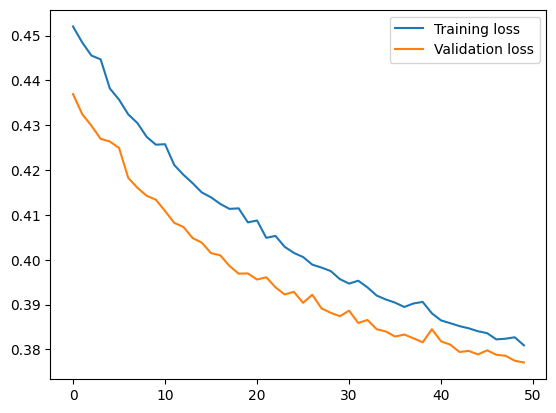
\includegraphics[width=0.75\textwidth]{ysa1.png}
    \caption{Çıktı Figürü}
    \label{fig:my_pic}
\end{figure}


\subsection{(10 Puan)} \textbf{SEED=öğrenci numaranız set ettikten sonra altıncı haftada ödev olarak verdiğim gibi earlystopping'deki en iyi modeli kullanarak, Prensesi İyileştir test setinden accuracy, F1, precision ve recall değerlerini hesaplayan kodu yazın ve sonucu da aşağı yapıştırın. \%80'den fazla başarı bekliyorum test setinden. Daha düşükse başarı oranınız, nerede hata yaptığınızı bulmaya çalışın. \%90'dan fazla başarı almak mümkün (ben denedim).}

\begin{python}
train_losses = []
val_losses = []
torch.manual_seed(190401056)

for epoch in range(num_epochs):
    model.train()
    train_loss = 0.0
    for batch_idx, (data, target) in enumerate(train_loader):
        optimizer.zero_grad()
        output = model(data)
        loss = criterion(output, target.squeeze())
        loss.backward()
        optimizer.step()
        train_loss += loss.item()
    train_losses.append(train_loss/len(train_loader))

    model.eval()
    val_loss = 0.0
    correct = 0
    total = 0
    with torch.no_grad():
        for data, target in valid_loader:
            output = model(data)
            loss = criterion(output, target.squeeze())
            val_loss += loss.item()
            _, predicted = torch.max(output.data, 1)
            total += target.size(0)
            correct += (predicted == target.squeeze()).sum().item()
        val_losses.append(val_loss/len(valid_loader))
    
    accuracy = 100 * correct / total
    print('Epoch: {}, Validation Accuracy: {:.2f}%'.format(epoch+1, accuracy))
 
    if accuracy > best_accuracy:
        best_accuracy = accuracy
        best_epoch = epoch
        torch.save(model.state_dict(), 'best_model.pt')
   
    elif epoch - best_epoch > patience:
        print(f'Early stopping: validation accuracy has not improved for {patience} epochs.')
        break

import matplotlib.pyplot as plt

plt.plot(train_losses, label='Training loss')
plt.plot(val_losses, label='Validation loss')
plt.legend()
plt.show()

best_model = MLP(input_size, hidden_size1, hidden_size2, output_size)

best_model.load_state_dict(torch.load("best_model.pt"))

best_model.eval()
from sklearn.metrics import classification_report
from sklearn.metrics import accuracy_score

best_model.eval()

test_loader = DataLoader(test_dataset, batch_size=len(test_dataset), shuffle=False)
X_test, y_test = next(iter(test_loader))

with torch.no_grad():
    output = best_model(X_test)
    _, predicted = torch.max(output.data, 1)

accuracy = accuracy_score(y_test.squeeze().numpy(), predicted.numpy()) * 100
report = classification_report(y_test.squeeze().numpy(), predicted.numpy(), target_names=["Not Saved", "Saved"])

print(f"Accuracy: {accuracy:.2f}%")
print(f"Classification Report:\n{report}")

\end{python}
Epoch: 1, Validation Accuracy: 95.22%

Epoch: 2, Validation Accuracy: 95.22%

Epoch: 3, Validation Accuracy: 95.22%

Epoch: 4, Validation Accuracy: 95.22%

Epoch: 5, Validation Accuracy: 95.22%

Epoch: 6, Validation Accuracy: 95.22%

Epoch: 7, Validation Accuracy: 95.22%

Early stopping: validation accuracy has not improved for 5 epochs.

\begin{figure}[ht!]
    \centering
    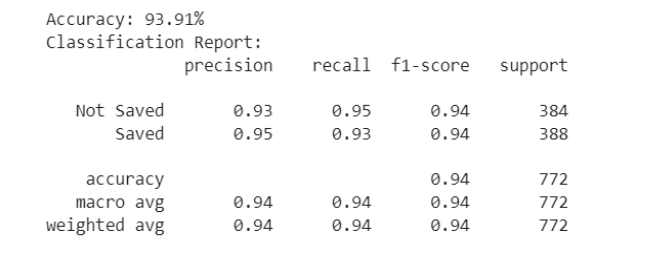
\includegraphics[width=0.75\textwidth]{ysa2.png}
    \caption{Çıktı }
    \label{fig:my_pic}
\end{figure}



\subsection{(5 Puan)} \textbf{Tüm kodların CPU'da çalışması ne kadar sürüyor hesaplayın. Sonra to device yöntemini kullanarak modeli ve verileri GPU'ya atıp kodu bir de böyle çalıştırın ve ne kadar sürdüğünü hesaplayın. Süreleri aşağıdaki tabloya koyun. GPU için Google Colab ya da Kaggle'ı kullanabilirsiniz, iki ortam da her hafta saatlerce GPU hakkı veriyor.}

\begin{table}[ht!]
    \centering
    \caption{Buraya bir açıklama yazın}
    \begin{tabular}{c|c}
        Ortam & Süre (saniye) \\\hline
        CPU & 12.976426124572754  \\
        GPU & 16.56697965567\\
    \end{tabular}
    \label{tab:my_table}
\end{table}

\subsection{(3 Puan)} \textbf{Modelin eğitim setine overfit etmesi için elinizden geldiği kadar kodu gereken şekilde değiştirin, validasyon loss'unun açıkça yükselmeye başladığı, training ve validation loss'ları içeren figürü aşağı koyun ve overfit için yaptığınız değişiklikleri aşağı yazın. Overfit, tam bir çanak gibi olmalı ve yükselmeli. Ona göre parametrelerle oynayın.}

Cevaplar buraya

% Figür aşağı
\begin{comment}
\begin{figure}[ht!]
    \centering
    \includegraphics[width=0.75\textwidth]{mypicturehere.png}
    \caption{Buraya açıklama yazın}
    \label{fig:my_pic}
\end{figure}
\end{comment}

\subsection{(2 Puan)} \textbf{Beşinci soruya ait tüm kodların ve cevapların olduğu jupyter notebook'un Github linkini aşağıdaki url'e koyun.}

\url{https://github.com/nurayaaltug/MultilayerPerceptron}

\section{(Toplam 10 Puan)} \textbf{Bir önceki sorudaki Prensesi İyileştir problemindeki yapay sinir ağınıza seçtiğiniz herhangi iki farklı regülarizasyon yöntemi ekleyin ve aşağıdaki soruları cevaplayın.} 

\subsection{(2 puan)} \textbf{Kodlarda regülarizasyon eklediğiniz kısımları aşağı koyun:} 

\begin{python}
kod_buraya = None
if kod_buraya:
    devam_ise_buraya = 0

print(devam_ise_buraya)
\end{python}

\subsection{(2 puan)} \textbf{Test setinden yeni accuracy, F1, precision ve recall değerlerini hesaplayıp aşağı koyun:}

Sonuçlar buraya.

\subsection{(5 puan)} \textbf{Regülarizasyon yöntemi seçimlerinizin sebeplerini ve sonuçlara etkisini yorumlayın:}

Yorumlar buraya.

\subsection{(1 puan)} \textbf{Sonucun github linkini  aşağıya koyun:}

\url{www.benimgithublinkim2.com}

\end{document}